\section{Examples}
\subsection{The tangent bundle of the 2-sphere}
\begin{itemize}
\item Define \( \oo \) via skeleta with inclusions. Use the inclusions to help identify aspects of the map \( \oo\to\BAutoso \).
\item Make it a lemma that \( \oo \) is the triple join
\item Define polytopes
\end{itemize}

The usual HoTT \( S^1 \) and \( S^2 \) are a little impoverished, and seeing connections and curvature is difficult. Instead we will define equivalent HITs that have more constructors. The representation of the sphere will be the octohedron \( \oo \) and the circle will be \( C_4 \) which has four points and is designed to work well with \( \oo \).

The Rubik's cube has a convenient standardized arrangement of colors that start with different letters (white, yellow, blue, orange, green, red) so we will use those to label our points, especially since having such a cube handy is very helpful to visualize some of the geometry that is encoded below as mere lists of data.

Should the 0-dimensional constructors represent the corners or the faces? We have so far found it intuitive to imagine taking the nerve of a good open cover, where the top-dimensional bulk of the cube, namely the faces, is converted to a point since an open set covering that face is contractible. That's why we end up with an icosohedron, which is a dual polyhedron to the cube.

We won't discuss in detail the fact that Mike Shulman's shape operator \cite{shulman_cohesion} is equivalent to taking the nerve of an open cover and forming a HIT from the overlap data. The shape operator preserves colimits and so the simple homotopy pushouts we are considering should be within the use cases of shape.

The HIT \( \oo \) is built from the following constructors:
\begin{enumerate}
\item Dimension 0: the vertices \( \{w, y, b, g, r, o, y\} \) where we think of \( w \) as the north pole and \( y \) the south pole.
\item Dimension 1: the 12 adjacency pairs of faces, denoted \( \{wb\}, \{wo\}  \) and so on.
\item Dimension 2: the set of faces generated by the 3-way adjacency of faces (which takes place in neighborhoods of the cube's original corners), denoted \( \{wbo\}, \{wog\} \) and so on.
\end{enumerate}

\begin{figure}[h]
\centering
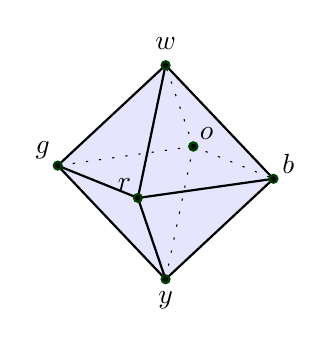
\begin{tikzpicture}%
  [x={(-0.860769cm, -0.121512cm)},
  y={(0.508996cm, -0.205391cm)},
  z={(-0.000053cm, 0.971107cm)},
  scale=1,
  back/.style={loosely dotted, thin},
  edge/.style={black, thick},
  facet/.style={fill=blue!95!black,fill opacity=0.1},
  vertex/.style={inner sep=1pt,circle,draw=green!25!black,fill=black,thick}]
\coordinate (-1, -1, 0) at (-1, -1, 0);
\coordinate (-1, 1, 0) at (-1, 1, 0);
\coordinate (0, 0, -1) at (0, 0, -1);
\coordinate (0, 0, 1) at (0, 0, 1);
\coordinate (1, -1, 0) at (1, -1, 0);
\coordinate (1, 1, 0) at (1, 1, 0);
%% Drawing edges in the back
%%
\draw[edge,back] (-1, -1, 0) -- (-1, 1, 0);
\draw[edge,back] (-1, -1, 0) -- (0, 0, -1.4);
\draw[edge,back] (-1, -1, 0) -- (0, 0, 1.4);
\draw[edge,back] (-1, -1, 0) -- (1, -1, 0);
%% Drawing vertices in the back
%%
\node[vertex] at (-1, -1, 0)     {};
%% Drawing the facets
%%
\fill[facet] (1, 1, 0) -- (0, 0, -1.4) -- (1, -1, 0) -- cycle {};
\fill[facet] (1, 1, 0) -- (0, 0, 1.4) -- (1, -1, 0) -- cycle {};
\fill[facet] (1, 1, 0) -- (-1, 1, 0) -- (0, 0, 1.4) -- cycle {};
\fill[facet] (1, 1, 0) -- (-1, 1, 0) -- (0, 0, -1.4) -- cycle {};
%% Drawing edges in the front
%%
\draw[edge] (-1, 1, 0) -- (0, 0, -1.4);
\draw[edge] (-1, 1, 0) -- (0, 0, 1.4);
\draw[edge] (-1, 1, 0) -- (1, 1, 0);
\draw[edge] (0, 0, -1.4) -- (1, -1, 0);
\draw[edge] (0, 0, -1.4) -- (1, 1, 0);
\draw[edge] (0, 0, 1.4) -- (1, -1, 0);
\draw[edge] (0, 0, 1.4) -- (1, 1, 0);
\draw[edge] (1, -1, 0) -- (1, 1, 0);
%% Drawing the vertices in the front
%%
\begin{scope}[nodes=vertex]
\node[label=above right:\( b \)] at (-1, 1, 0)     {};
\node[label=below:\( y \)] at (0, 0, -1.4)     {};
\node[label=above:\( w \)] at (0, 0, 1.4)     {};
\node[label=above left:\( g \)] at (1, -1, 0)     {};
\node[label=above left:\( r \)] at (1, 1, 0)     {};
\node[label=above right:\( o \)] at (-1, -1, 0)     {};
\end{scope}
\end{tikzpicture}
\caption{The HIT \( \oo \) which has 6 points, 12 1-paths, 8 2-paths.}
\end{figure}

We will choose a base point of \( \BAutoso \) that has four points, just like the equator of \( \oo \).

\begin{mydef}
Denote by \( C_4 \) the join \( \{b, g\}*\{r, o\} \). This is the equator of the discrete octahedral sphere. Then \( \oo \) itself can be seen as the join \( \{w, y\}* C_4 \).
\end{mydef}

\begin{figure}[h]
\centering
\begin{tikzpicture}[
node distance = 15mm and 15mm,
V/.style = {circle, fill, draw=black, inner sep=1pt, font=\footnotesize},
every edge quotes/.style = {auto, font=\footnotesize},
arrow/.style={->,semithick}
]
\begin{scope}[nodes=V]
  \node[label=above left:\( b \)] (1) {};
  \node[label=above right:\( r \)] (2) [right=of 1]  {};
  \node[label=below right:\( g \)] (3) [below=of 2]  {};
  \node[label=below left:\( o \)] (4) [below=of 1]  {};
\end{scope}
\draw[arrow]
        (1)  edge["\( br \)"] (2)
        (2)  edge["\( rg \)"] (3)
        (3)  edge["\( go \)"] (4)
        (4)  edge["\( ob \)"] (1);
\end{tikzpicture}
\caption{The HIT \( C_4 \) which is one of the types in \( \BAutoso \)}
\end{figure}

\begin{mylemma}
\( (C_4, b)\simeq S^1 \).
\end{mylemma}
\begin{proof}Similar to Lemma 6.5.1 from the HoTT book\cite{hottbook}. We will make some use of the particular map \( \{b, r, g, o\}\mapsto \mathsf{base}, br\mapsto \mathsf{loop}, \{rg, go, ob\}\mapsto \refl. \)\end{proof}

\begin{mylemma}
\( \oo\simeq S^2 \).
\end{mylemma}
\begin{proof}\( \oo \) is the join of \( C_4 \) and a two-point type. For more discussion of the join operation see the HoTT book section 8.5\cite{hottbook}.\end{proof}

To produce a term in \( \BAutoso \) we need \( C_4 \) and a choice of an equivalence class of equivalences with \( S^1 \):
\begin{mylemma}
We have \( (C_4, ||\{b, r, g, o\}\mapsto \mathsf{base}, br\mapsto \mathsf{loop}, \{rg, go, ob\}\mapsto \refl ||_0):\BAutoso \)
\end{mylemma}

There are other near-to-hand terms of \( \BAutoso \) we can denote like: \( [w, o, y, r] \), meaning the square isomorphic to \( C_4 \) but with the given four points, with pointing given by whichever point we listed first, and with equivalence with \( S^1 \) chosen so that the path between the first two points maps to \( \mathsf{loop} \). We will also introduce notation for maps \( f:[a, b, c, d]\to [w, x, y, z] \) by indicating where each item in the domain list is sent, like so: \( f\defeq[[x, y, z, w]] \).

\( C_4 \) has an unpointed automorphism connected to the identiy which will play the role of rotation by 90 degrees:

\begin{mydef}
Let \( R:C_4\to C_4 \) be the cyclic permutation given by \( R(b)=r, R(r)=g, R(g)=o, R(o)=b, R(br)=rg, R(rg)=go, R(go)=ob, R(ob)=br. \) Let \( R':R=\id \) be the obvious homotopy to the identity.
\end{mydef}

To construct a map \( \oo\to\BAutoso \) we need to send each vertex to an \( S^1 \)-torsor such as \( C_4 \). We will choose to send each vertex to ``the clockwise equator if this was the north pole.'' 

\begin{figure}[h]
\centering
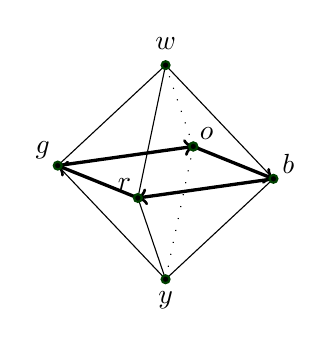
\begin{tikzpicture}%
  [x={(-0.860769cm, -0.121512cm)},
  y={(0.508996cm, -0.205391cm)},
  z={(-0.000053cm, 0.971107cm)},
  scale=1,
  eqback/.style={->, very thick},
  back/.style={loosely dotted, thin},
  eqedge/.style={->, very thick},
  edge/.style={black, thin},
  facet/.style={fill=blue!95!black,fill opacity=0.0},
  vertex/.style={inner sep=1pt,circle,draw=green!25!black,fill=black,thick}]
\coordinate (-1, -1, 0) at (-1, -1, 0);
\coordinate (-1, 1, 0) at (-1, 1, 0);
\coordinate (0, 0, -1) at (0, 0, -1);
\coordinate (0, 0, 1) at (0, 0, 1);
\coordinate (1, -1, 0) at (1, -1, 0);
\coordinate (1, 1, 0) at (1, 1, 0);
%% Drawing edges in the back
%%
\draw[edge,eqback] (-1, -1, 0) -- (-1, 1, 0);
\draw[edge,back] (-1, -1, 0) -- (0, 0, -1.4);
\draw[edge,back] (-1, -1, 0) -- (0, 0, 1.4);
\draw[edge,eqback] (1, -1, 0) -- (-1, -1, 0);
%% Drawing vertices in the back
%%
\node[vertex] at (-1, -1, 0)     {};
%% Drawing the facets
%%
\fill[facet] (1, 1, 0) -- (0, 0, -1.4) -- (1, -1, 0) -- cycle {};
\fill[facet] (1, 1, 0) -- (0, 0, 1.4) -- (1, -1, 0) -- cycle {};
\fill[facet] (1, 1, 0) -- (-1, 1, 0) -- (0, 0, 1.4) -- cycle {};
\fill[facet] (1, 1, 0) -- (-1, 1, 0) -- (0, 0, -1.4) -- cycle {};
%% Drawing edges in the front
%%
\draw[edge] (-1, 1, 0) -- (0, 0, -1.4);
\draw[edge] (-1, 1, 0) -- (0, 0, 1.4);
\draw[eqedge] (-1, 1, 0) -- (1, 1, 0);
\draw[edge] (0, 0, -1.4) -- (1, -1, 0);
\draw[edge] (0, 0, -1.4) -- (1, 1, 0);
\draw[edge] (0, 0, 1.4) -- (1, -1, 0);
\draw[edge] (0, 0, 1.4) -- (1, 1, 0);
\draw[eqedge] (1, 1, 0) -- (1, -1, 0);
%% Drawing the vertices in the front
%%
\begin{scope}[nodes=vertex]
\node[label=above right:\( b \)] at (-1, 1, 0)     {};
\node[label=below:\( y \)] at (0, 0, -1.4)     {};
\node[label=above:\( w \)] at (0, 0, 1.4)     {};
\node[label=above left:\( g \)] at (1, -1, 0)     {};
\node[label=above left:\( r \)] at (1, 1, 0)     {};
\node[label=above right:\( o \)] at (-1, -1, 0)     {};
\end{scope}
\end{tikzpicture}

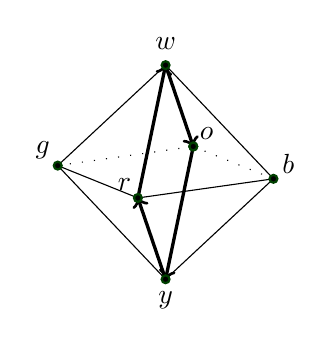
\begin{tikzpicture}%
  [x={(-0.860769cm, -0.121512cm)},
  y={(0.508996cm, -0.205391cm)},
  z={(-0.000053cm, 0.971107cm)},
  scale=1,
  eqback/.style={->, very thick},
  back/.style={loosely dotted, thin},
  eqedge/.style={->, very thick},
  edge/.style={black, thin},
  facet/.style={fill=blue!95!black,fill opacity=0.0},
  vertex/.style={inner sep=1pt,circle,draw=green!25!black,fill=black,thick}]
\coordinate (-1, -1, 0) at (-1, -1, 0);
\coordinate (-1, 1, 0) at (-1, 1, 0);
\coordinate (0, 0, -1) at (0, 0, -1);
\coordinate (0, 0, 1) at (0, 0, 1);
\coordinate (1, -1, 0) at (1, -1, 0);
\coordinate (1, 1, 0) at (1, 1, 0);
%% Drawing edges in the back
%%
\draw[edge,back] (-1, -1, 0) -- (-1, 1, 0);
\draw[edge,eqback] (-1, -1, 0) -- (0, 0, -1.4);
\draw[edge,eqback] (0, 0, 1.4) -- (-1, -1, 0);
\draw[edge,back] (1, -1, 0) -- (-1, -1, 0);
%% Drawing vertices in the back
%%
\node[vertex] at (-1, -1, 0)     {};
%% Drawing the facets
%%
\fill[facet] (1, 1, 0) -- (0, 0, -1.4) -- (1, -1, 0) -- cycle {};
\fill[facet] (1, 1, 0) -- (0, 0, 1.4) -- (1, -1, 0) -- cycle {};
\fill[facet] (1, 1, 0) -- (-1, 1, 0) -- (0, 0, 1.4) -- cycle {};
\fill[facet] (1, 1, 0) -- (-1, 1, 0) -- (0, 0, -1.4) -- cycle {};
%% Drawing edges in the front
%%
\draw[edge] (-1, 1, 0) -- (0, 0, -1.4);
\draw[edge] (-1, 1, 0) -- (0, 0, 1.4);
\draw[edge] (-1, 1, 0) -- (1, 1, 0);
\draw[edge] (0, 0, -1.4) -- (1, -1, 0);
\draw[eqedge] (0, 0, -1.4) -- (1, 1, 0);
\draw[edge] (0, 0, 1.4) -- (1, -1, 0);
\draw[eqedge] (1, 1, 0) -- (0, 0, 1.4) ;
\draw[edge] (1, 1, 0) -- (1, -1, 0);
%% Drawing the vertices in the front
%%
\begin{scope}[nodes=vertex]
\node[label=above right:\( b \)] at (-1, 1, 0)     {};
\node[label=below:\( y \)] at (0, 0, -1.4)     {};
\node[label=above:\( w \)] at (0, 0, 1.4)     {};
\node[label=above left:\( g \)] at (1, -1, 0)     {};
\node[label=above left:\( r \)] at (1, 1, 0)     {};
\node[label=above right:\( o \)] at (-1, -1, 0)     {};
\end{scope}
\end{tikzpicture}

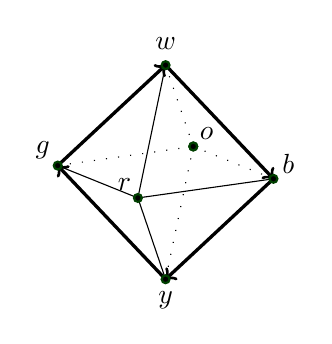
\begin{tikzpicture}%
  [x={(-0.860769cm, -0.121512cm)},
  y={(0.508996cm, -0.205391cm)},
  z={(-0.000053cm, 0.971107cm)},
  scale=1,
  eqback/.style={->, very thick},
  back/.style={loosely dotted, thin},
  eqedge/.style={->, very thick},
  edge/.style={black, thin},
  facet/.style={fill=blue!95!black,fill opacity=0.0},
  vertex/.style={inner sep=1pt,circle,draw=green!25!black,fill=black,thick}]
\coordinate (-1, -1, 0) at (-1, -1, 0);
\coordinate (-1, 1, 0) at (-1, 1, 0);
\coordinate (0, 0, -1) at (0, 0, -1);
\coordinate (0, 0, 1) at (0, 0, 1);
\coordinate (1, -1, 0) at (1, -1, 0);
\coordinate (1, 1, 0) at (1, 1, 0);
%% Drawing edges in the back
%%
\draw[edge,back] (-1, -1, 0) -- (-1, 1, 0);
\draw[edge,back] (-1, -1, 0) -- (0, 0, -1.4);
\draw[edge,back] (-1, -1, 0) -- (0, 0, 1.4);
\draw[edge,back] (1, -1, 0) -- (-1, -1, 0);
%% Drawing vertices in the back
%%
\node[vertex] at (-1, -1, 0)     {};
%% Drawing the facets
%%
\fill[facet] (1, 1, 0) -- (0, 0, -1.4) -- (1, -1, 0) -- cycle {};
\fill[facet] (1, 1, 0) -- (0, 0, 1.4) -- (1, -1, 0) -- cycle {};
\fill[facet] (1, 1, 0) -- (-1, 1, 0) -- (0, 0, 1.4) -- cycle {};
\fill[facet] (1, 1, 0) -- (-1, 1, 0) -- (0, 0, -1.4) -- cycle {};
%% Drawing edges in the front
%%
\draw[eqedge] (-1, 1, 0) -- (0, 0, -1.4);
\draw[eqedge] (0, 0, 1.4) -- (-1, 1, 0);
\draw[edge] (-1, 1, 0) -- (1, 1, 0);
\draw[eqedge] (0, 0, -1.4) -- (1, -1, 0);
\draw[edge] (0, 0, -1.4) -- (1, 1, 0);
\draw[eqedge] (1, -1, 0) -- (0, 0, 1.4);
\draw[edge] (0, 0, 1.4) -- (1, 1, 0);
\draw[edge] (1, 1, 0) -- (1, -1, 0);
%% Drawing the vertices in the front
%%
\begin{scope}[nodes=vertex]
\node[label=above right:\( b \)] at (-1, 1, 0)     {};
\node[label=below:\( y \)] at (0, 0, -1.4)     {};
\node[label=above:\( w \)] at (0, 0, 1.4)     {};
\node[label=above left:\( g \)] at (1, -1, 0)     {};
\node[label=above left:\( r \)] at (1, 1, 0)     {};
\node[label=above right:\( o \)] at (-1, -1, 0)     {};
\end{scope}
\end{tikzpicture}
\caption{The equators for \( w, b, r \).}
\end{figure}

\begin{mydef}
Define \( T_0:\oo\to\BAutoso \) on just the 0-skeleton by
\begin{itemize}
\item \( T_0(b)=[w, o, y, r] \).
\item \( T_0(o)=[w, g, y, b] \).
\item \( T_0(g)=[w, r, y, o] \).
\item \( T_0(r)=[w, b, y, g] \).
\item \( T_0(w)=[b, r, g, o] \).
\item \( T_0(y)=[b, o, g, r] \).
\end{itemize}
\end{mydef}

Extending this to the 1-skeleton requires various choices. We will choose the one that reflects the tangent bundle, using the transport we can intuitively see through the embedding of \( \oo \) in 3-dimensional space as in our pictures. If you focus for a moment just on a path \( w\to b\to r \) and imagine rigidly tipping a moving equator along with a moving point, you can imagine a moving-equator point that starts at \( r \) and stays fixed when the north pole slides from \( w \) to \( b \). When the north pole continues sliding from \( b \) to \( r \) the moving-equator point moves to \( g \). Then it remains fixed when the north pole slides from \( r \) up to \( w \). So all in all we ``moved \( r \) to \( g \).'' When we track all the points on the original \( w \)-equator we see that we performed the rotation we earlier named \( R \).

In general we have:
\begin{mydef}
Define \( T_1:\oo\to\BAutoso \) on just the 1-skeleton by extending \( T_0 \) as follows:
Transport away from \( w \):
\begin{itemize}
\item \( T_1(wb):[b, r, g, o]\mapsto [y, r, w, o] \) (\( r, o \) fixed)
\item \( T_1(wr):[b, r, g, o]\mapsto [b, y, g, w] \) (\( b, g \) fixed)
\item \( T_1(wg):[b, r, g, o]\mapsto [w, r, y, o] \)
\item \( T_1(wo):[b, r, g, o]\mapsto [b, w, g, y] \)
\end{itemize}
Transport away from \( y \):
\begin{itemize}
\item \( T_1(yb):[b, o, g, r]\mapsto [w, o, y, r] \)
\item \( T_1(yr):[b, o, g, r]\mapsto [b, y, g, w] \)
\item \( T_1(yg):[b, o, g, r]\mapsto [y, o, w, r] \)
\item \( T_1(yo):[b, o, g, r]\mapsto [b, w, g, y] \)
\end{itemize}
Transport along the equator:
\begin{itemize}
\item \( T_1(br):[w, o, y, r]\mapsto [w, b, y, g] \) 
\item \( T_1(rg):[w, b, y, g]\mapsto [w, r, y, o] \)
\item \( T_1(go):[w, r, y, o]\mapsto [w, g, y, b] \)
\item \( T_1(ob):[w, g, y, b]\mapsto [w, o, y, r] \)
\end{itemize}
\end{mydef}

At this point we have defined a map on the 1-skeleton of \( \oo \).

\begin{myclaim}
\( T_1 \) defines a principal circle bundle with connection over the 1-skeleton of \( \oo \).
\end{myclaim}

We now want to extend this map to all of \( \oo \) by providing values for the eight faces. Here we will be guided by the classical relationship between a connection and its curvature. The curvature is computed from the connection, it doesn't contain any new data. Classically the integral of curvature over a 2-cell is the holonomy given by transport around the boundary. 

\begin{mydef}
Define \( T_2:\oo\to\BAutoso \) by extending \( T_1 \) as follows. We will send every clockwise triangle to \( R' \), the homotopy from \( \refl \) to \( R \):
\begin{itemize}
\item \( T_2(wbr)=R' \) 
\item \( T_2(wrg)=R' \)
\item \( T_2(wgo)=R' \)
\item \( T_2(ybo)=R' \)
\item \( T_2(yrb)=R' \) 
\item \( T_2(ygr)=R' \)
\item \( T_2(yog)=R' \)
\item \( T_2(ybo)=R' \)
\end{itemize}
\end{mydef}


\subsection{Combinatorial manifolds}

(This section is not quite off the ground.)

The combinatorial structure we have in mind is a nerve of a good open cover. What do we know about which smooth manifolds have such covers? While we're at it, let's survey all the combinatorial-flavored spaces and survey what smooth manifolds are homotopy equivalent to which structures.

What topological manifolds are equivalent to a CW complex? The answer is the composition of a few results summarized by Allen Hatcher\footnote{\url{https://mathoverflow.net/questions/201944/topological-n-manifolds-have-the-homotopy-type-of-n-dimensional-cw-complexes}} (citing \cite{kirby_siebenmann} and \cite{freedman_quinn}):

\begin{quote}
Every topological manifold has a handlebody structure except in dimension 4, where a 4-manifold has a handlebody structure if and only if it is smoothable. This is a theorem on page 136 of Freedman and Quinn's book ``Topology of 4-Manifolds'', with a reference given to the Kirby-Siebenmann book for the higher-dimensional case. It is then an elementary fact that an \( n \)-manifold with a handlebody structure is homotopy equivalent to a CW complex with one \( k \)-cell for each \( k \)-handle, so in particular there are no cells of dimension greater than \( n \). At least in the compact case a manifold with a handlebody structure is in fact homeomorphic to a CW complex with \( k \)-cells corresponding to \( k \)-handles; see page 107 of Kirby-Siebenmann. This probably holds in the noncompact case as well, though I don't know a reference.
\end{quote}


